%%% section Design and Implementation: Truck
\section{Design and Implementation: Truck}
\label{sec:design and implementation_truck} 

The truck consists of 3 main components, Controller, Driver interface and Communication module as shown in Figure \ref{img:truck_architecture}. We treat Truck as a whole component that will be run through an ‘.exe’ file. All the main components of the Truck are executed as threads to ensure concurrency, this way we can have some parallelism in the implementation. This behavior is visualized in Figure \ref{img:truck_activity}. Those components will be explained in detail in the incoming sub-section.
  
%%% image truck architecture
\begin{figure}[ht]
    \centering
    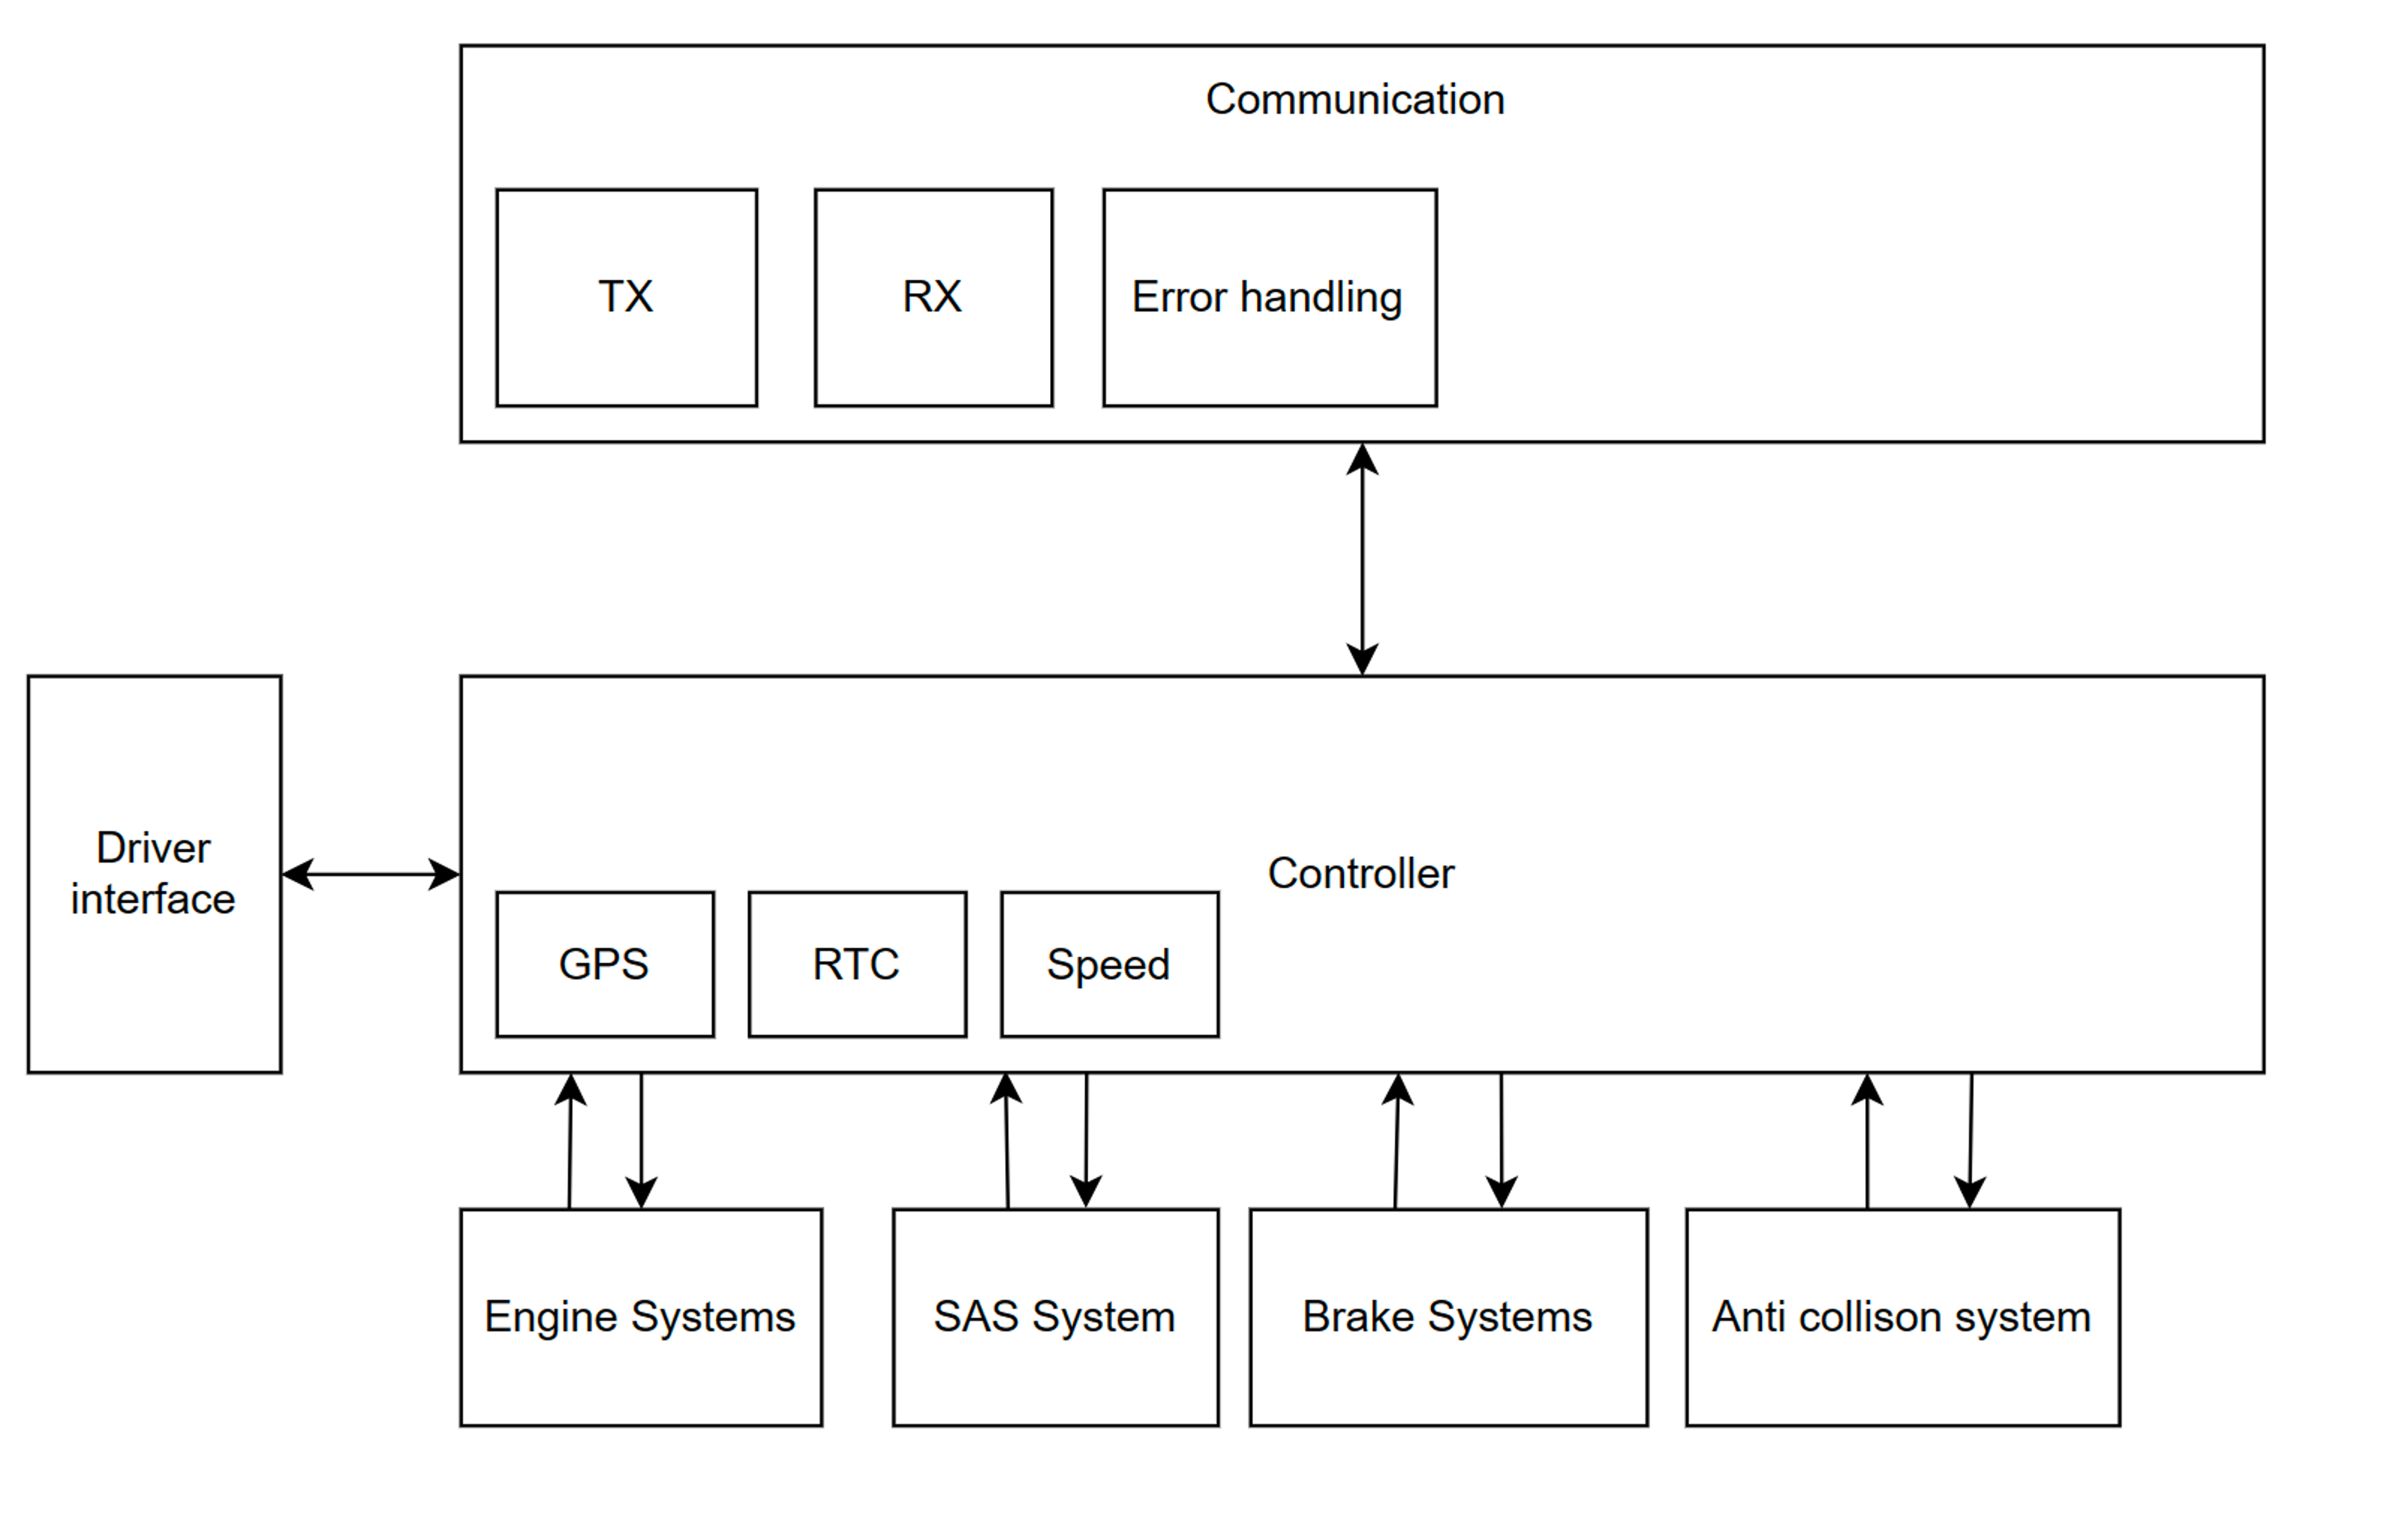
\includegraphics[width=0.5\textwidth]{images/truck_architecture.png}
    \caption{Truck Architecture}
    \label{img:truck_architecture}
\end{figure}

%%% image parallel process (truck activity)
\begin{figure}[ht]
    \centering
    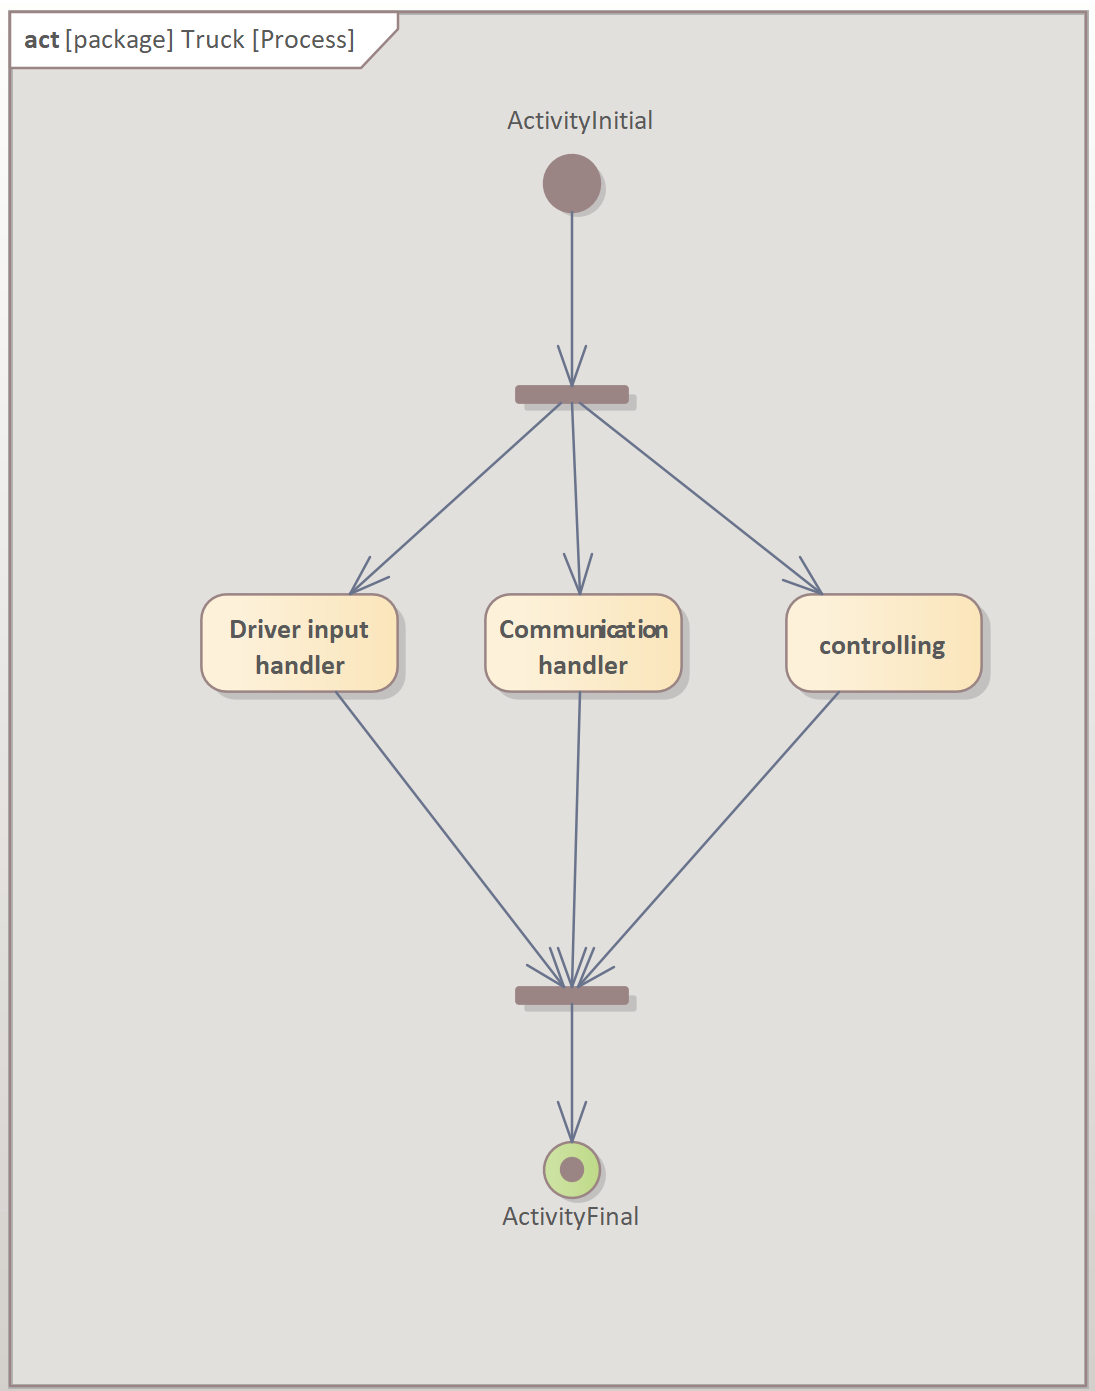
\includegraphics[width=0.3\textwidth]{images/truck_activity.png}
    \caption{Main process run by the truck}
    \label{img:truck_activity}
\end{figure}

%%% subsection controller
\subsection{Controller}
\label{subsec:controller} 

The controller is the main component that controls the behavior of the truck, and the other component or sub system is the output or input to the controller. The behavior is modeled as in Figure \ref{img:controller_state_machine} where it has 5 main states, Initial, waiting, leader, follower and system stop state. The state machine is implemented using switch case as in Listing \ref{code:code_satemachine}

%%% image controller state machine
\begin{figure}[ht]
    \centering
    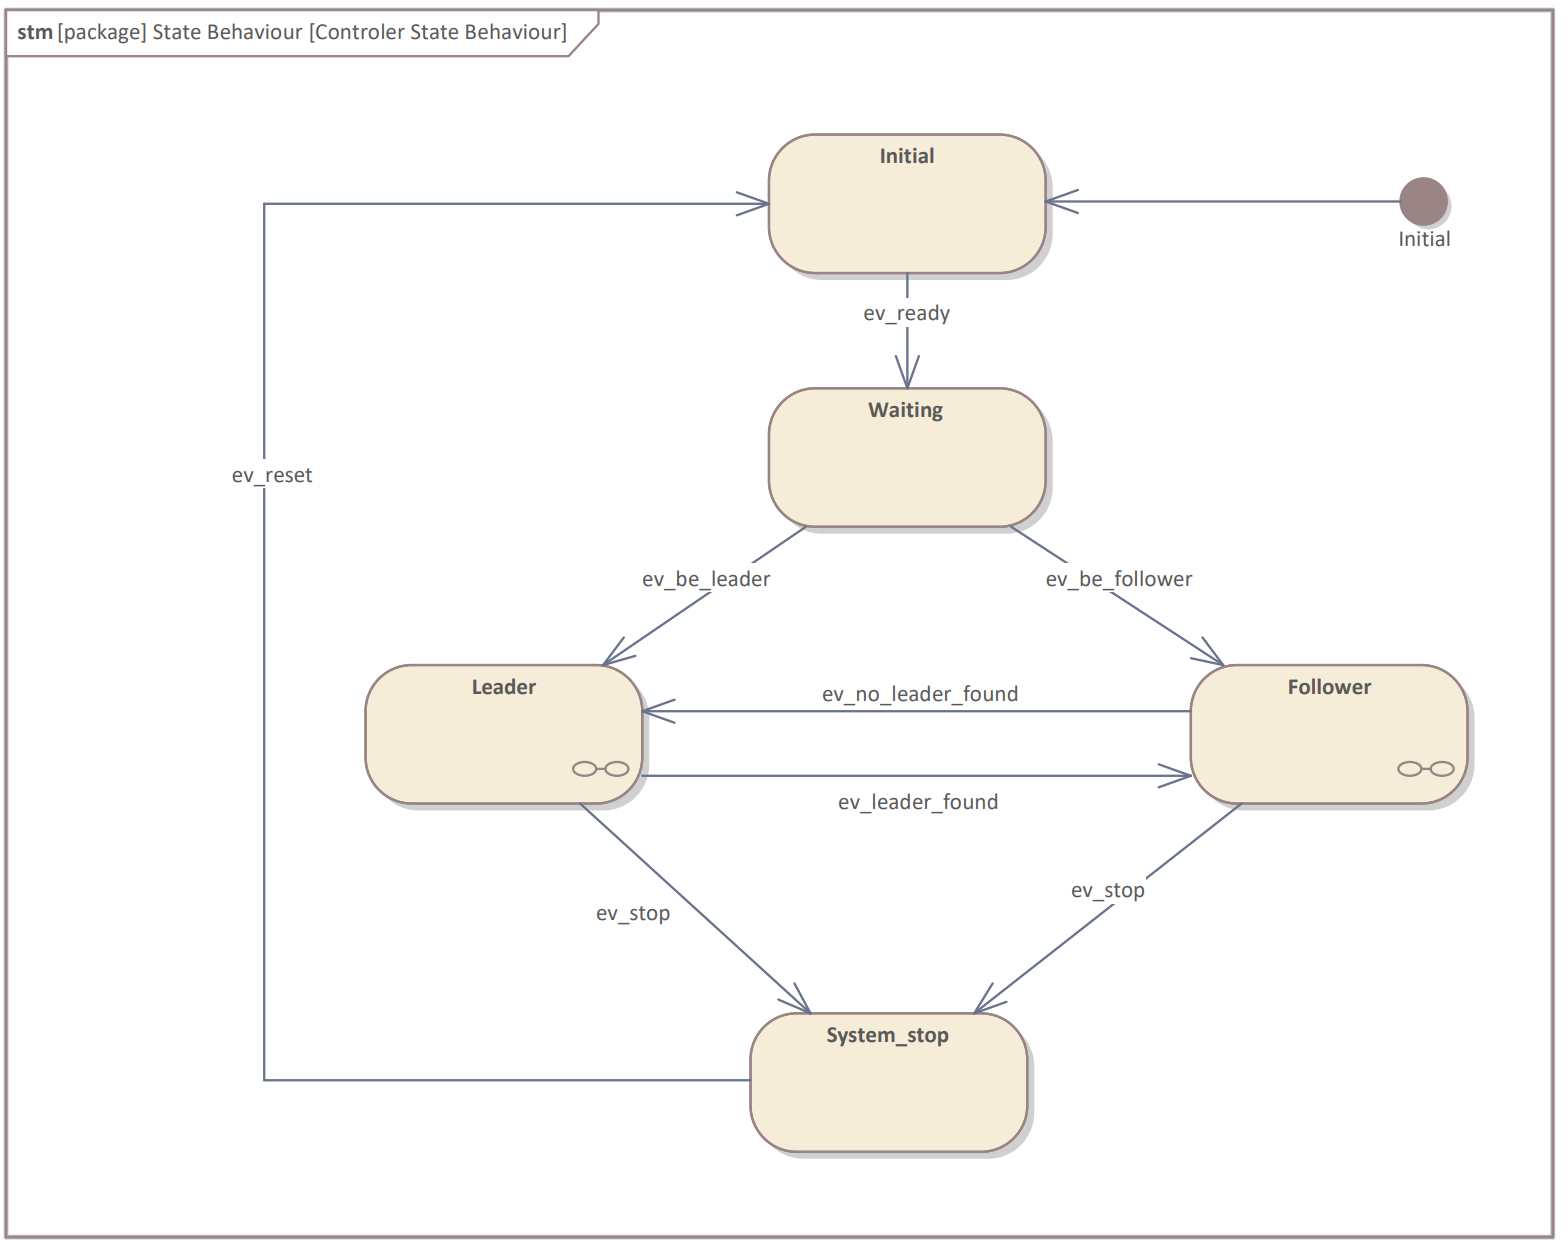
\includegraphics[width=0.5\textwidth]{images/controller_state_machine.png}
    \caption{Controller State Machine}
    \label{img:controller_state_machine}
\end{figure}

The reason it has leader and follower state is because the truck can change its roles while still active or moving. The leader and follower state have its own internal state as depict in Figure \ref{img:leader_state_machine} and Figure \ref{img:follower_state_machine}, where both have a moving state, error handling state and emergency stop state and only follower state have align state because it need to keep align with its leader.

%%% image leader state machine
\begin{figure}[ht]
    \centering
    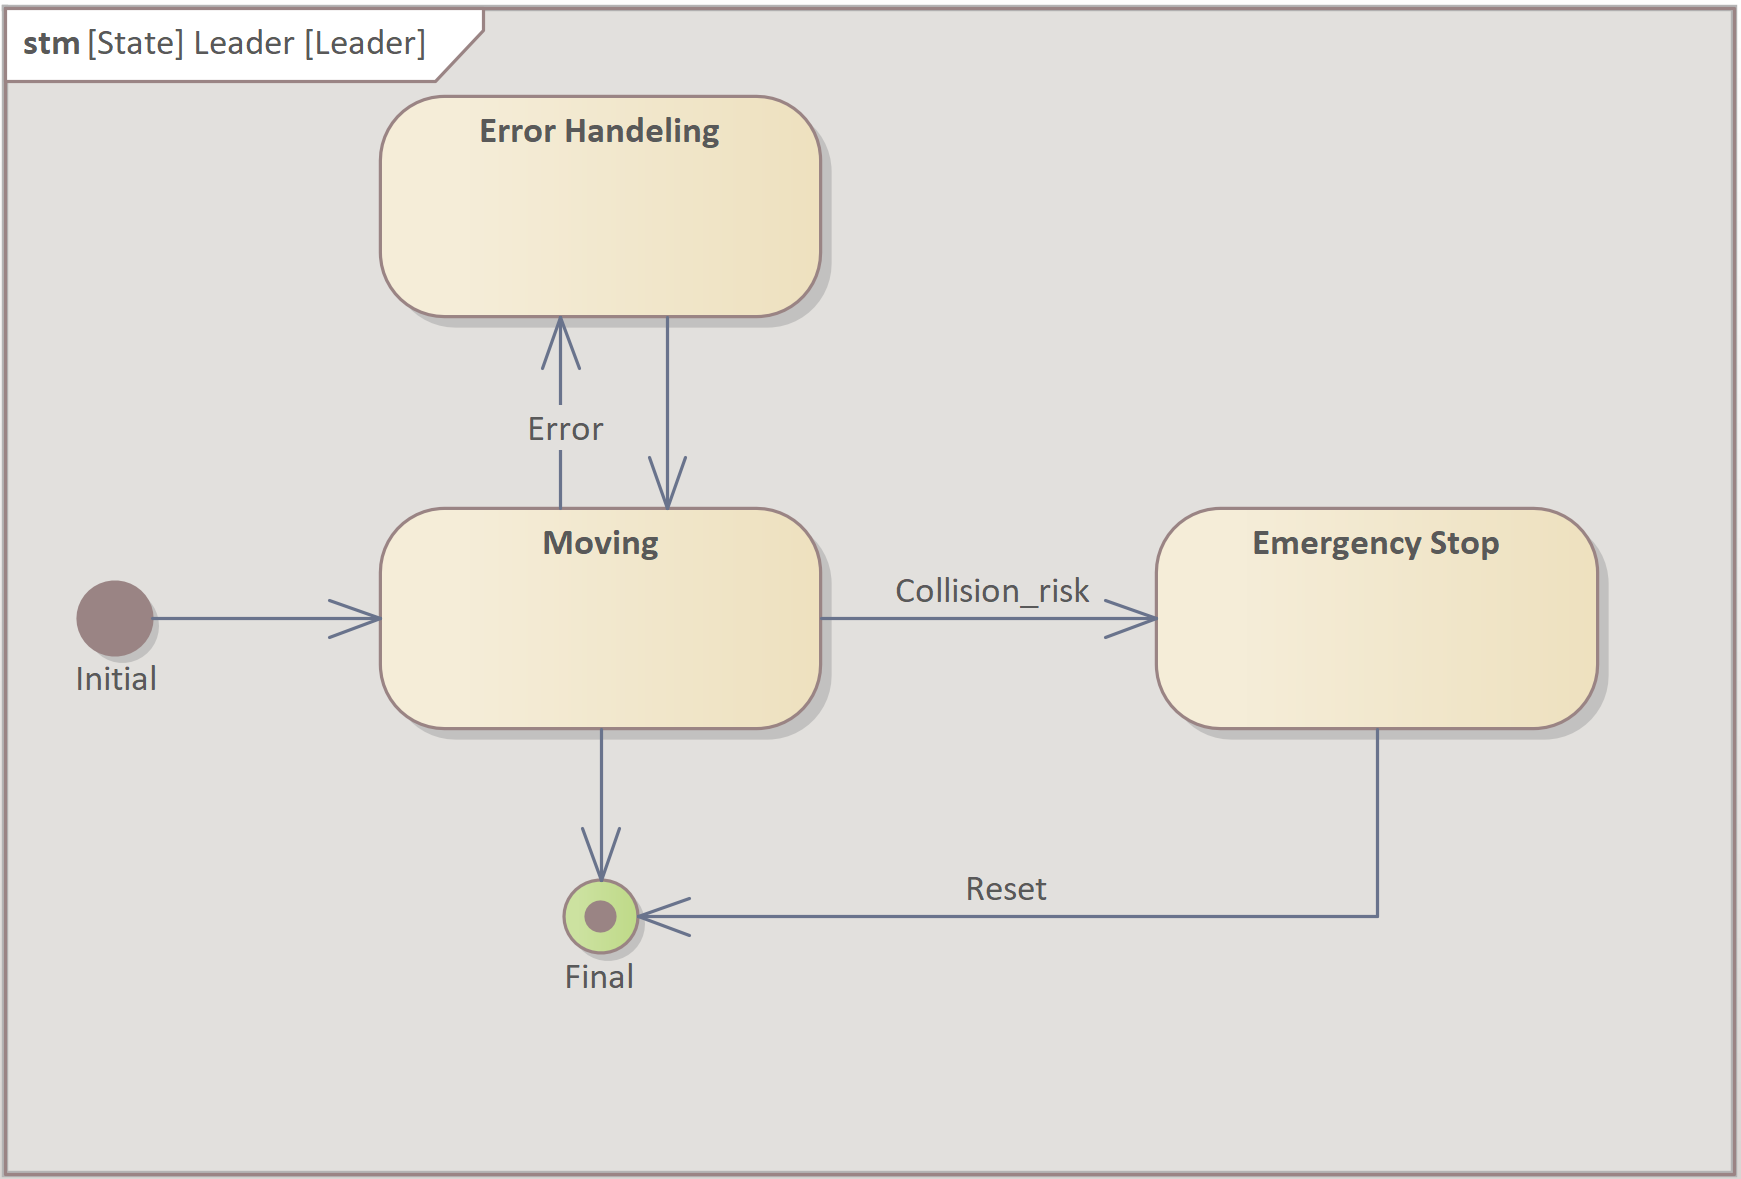
\includegraphics[width=0.4\textwidth]{images/leader_state_machine.png}
    \caption{Internal state machine of leader state}
    \label{img:leader_state_machine}
\end{figure}


%%% image follower state machine
\begin{figure}[ht]
    \centering
    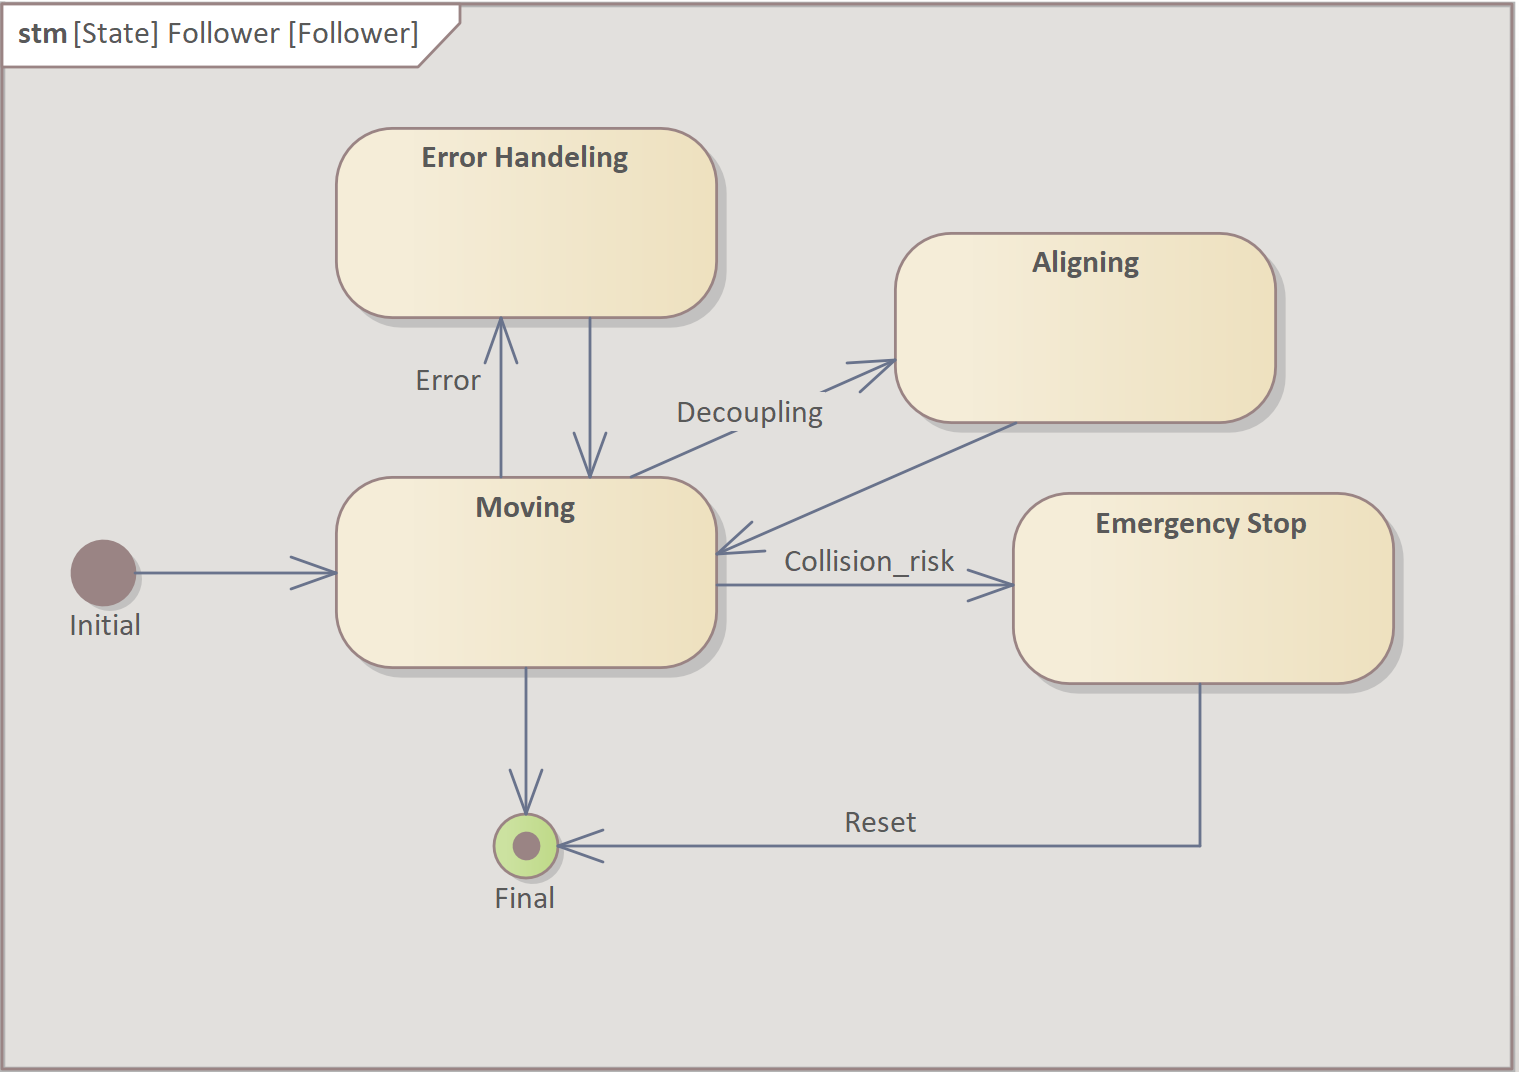
\includegraphics[width=0.4\textwidth]{images/follower_state_machine.png}
    \caption{ Internal state machine of follower state }
    \label{img:follower_state_machine}
\end{figure}

Based on Figure \ref{img:controller_state_machine}, Figure \ref{img:leader_state_machine} and \ref{img:follower_state_machine}, most of the transition is influenced by an event or a signal. For instance, from waiting state, it will change to leader state if and only if it receives a leader signal and and it will change to follower state if and only if it receives follower signal. Those signals could be produced by the controller itself or another component within the suck such as communication module.
The controller behaves differently in each state. In initial state, the controller will initialize all subsystems and produce a ready signal after that as visualized in Figure \ref{img:initial_state_activity}. The signal will trigger the transition from initial state to the waiting state. In a waiting state, the role of the truck will be decided by finding the leader. If a leader is found, it will set it role to follower and produce follower signal otherwise, it will be a leader and produce leader signal as shown in Figure \ref{img:waiting_state_activity}. Find a leader means that the truck tries to find another nearest front truck. 
%%% image initial state activity
\begin{figure}[ht]
    \centering
    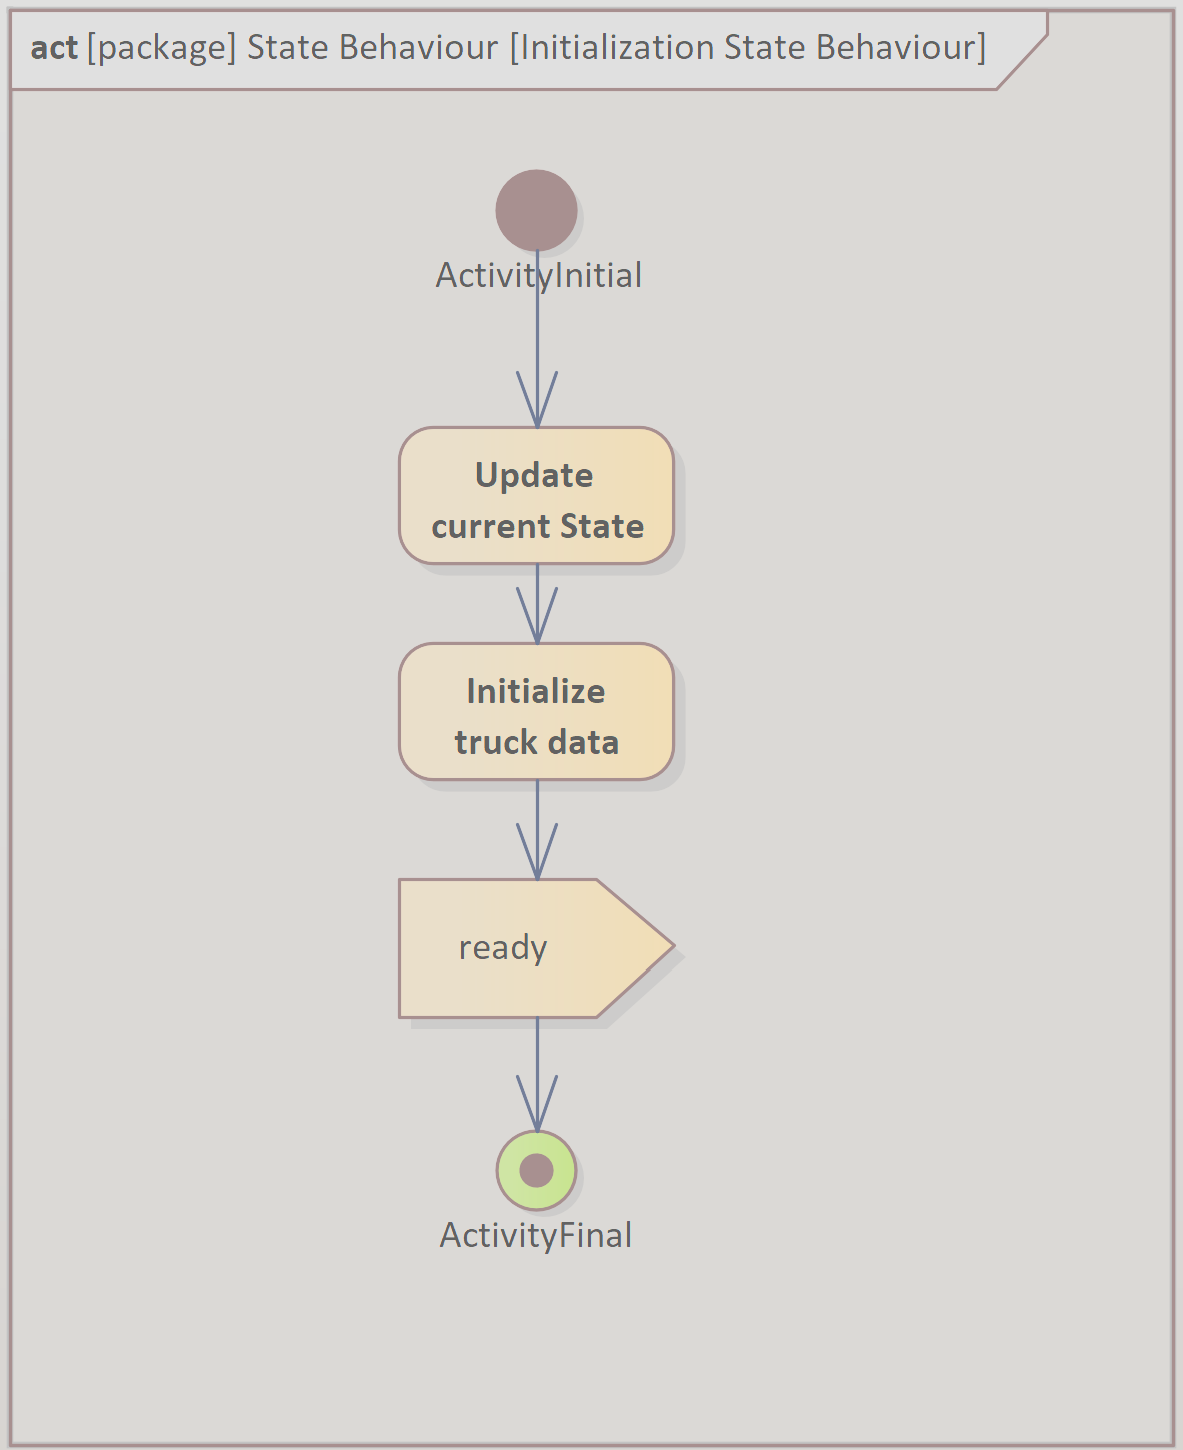
\includegraphics[width=0.3\textwidth]{images/initial_state_activity.png}
    \caption{ Initial state behaviour}
    \label{img:initial_state_activity}
\end{figure}


%%% image waiting state activity
\begin{figure}[ht]
    \centering
    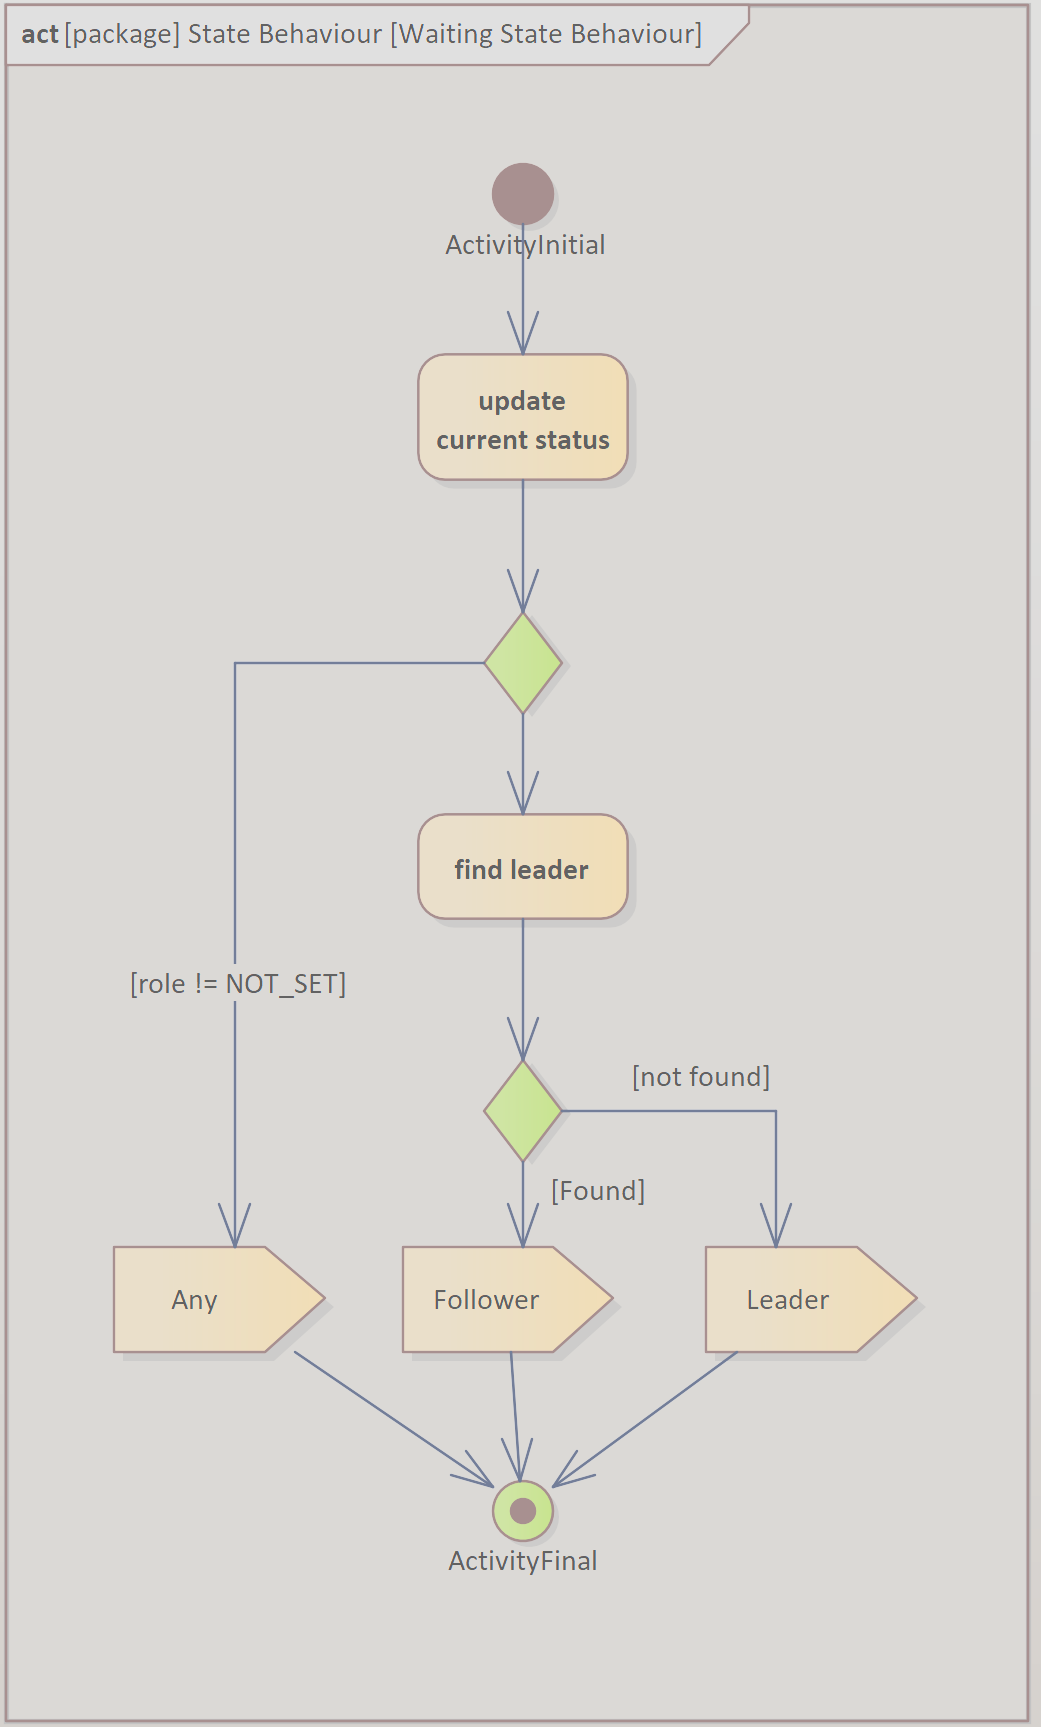
\includegraphics[width=0.3\textwidth]{images/waiting_state_activity.png}
    \caption{ Waiting state behaviour}
    \label{img:waiting_state_activity}
\end{figure}


The event from waiting state will decide whether it will enter the leader state or follower state.  Both internal states will start with moving state as in Figure \ref{img:leader_state_activity} and \ref{img:follower_state activity}. As leader, it will always send its movement set either by a driver or the system itself to the follower. Every new movement it increments its logical clock that is also shared to its follower and a routine to check for new event is executed. 
%%% image leader state activity
\begin{figure}[ht]
    \centering
    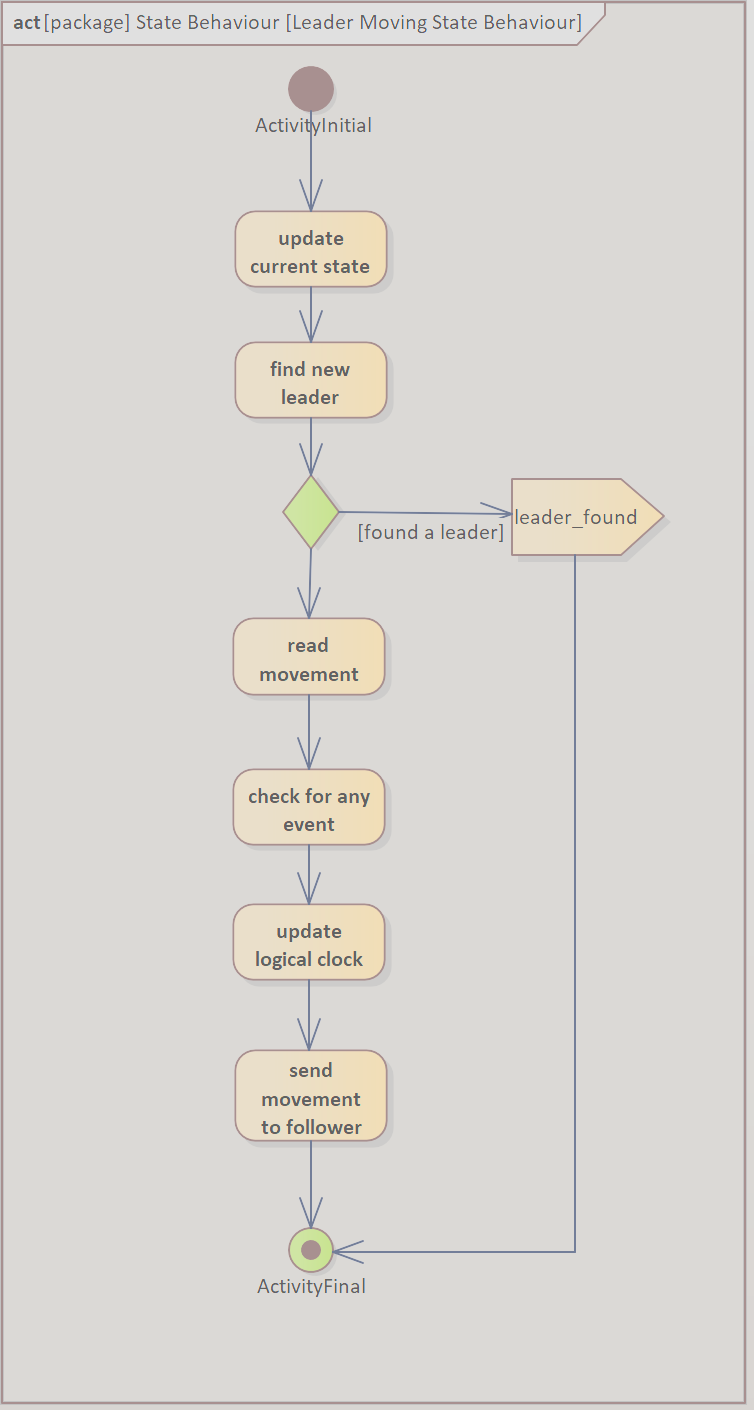
\includegraphics[width=0.3\textwidth]{images/leader_state_activity.png}
    \caption{ leader state behaviour}
    \label{img:leader_state_activity}
\end{figure}


%%% image follower state activity
\begin{figure}[ht]
    \centering
    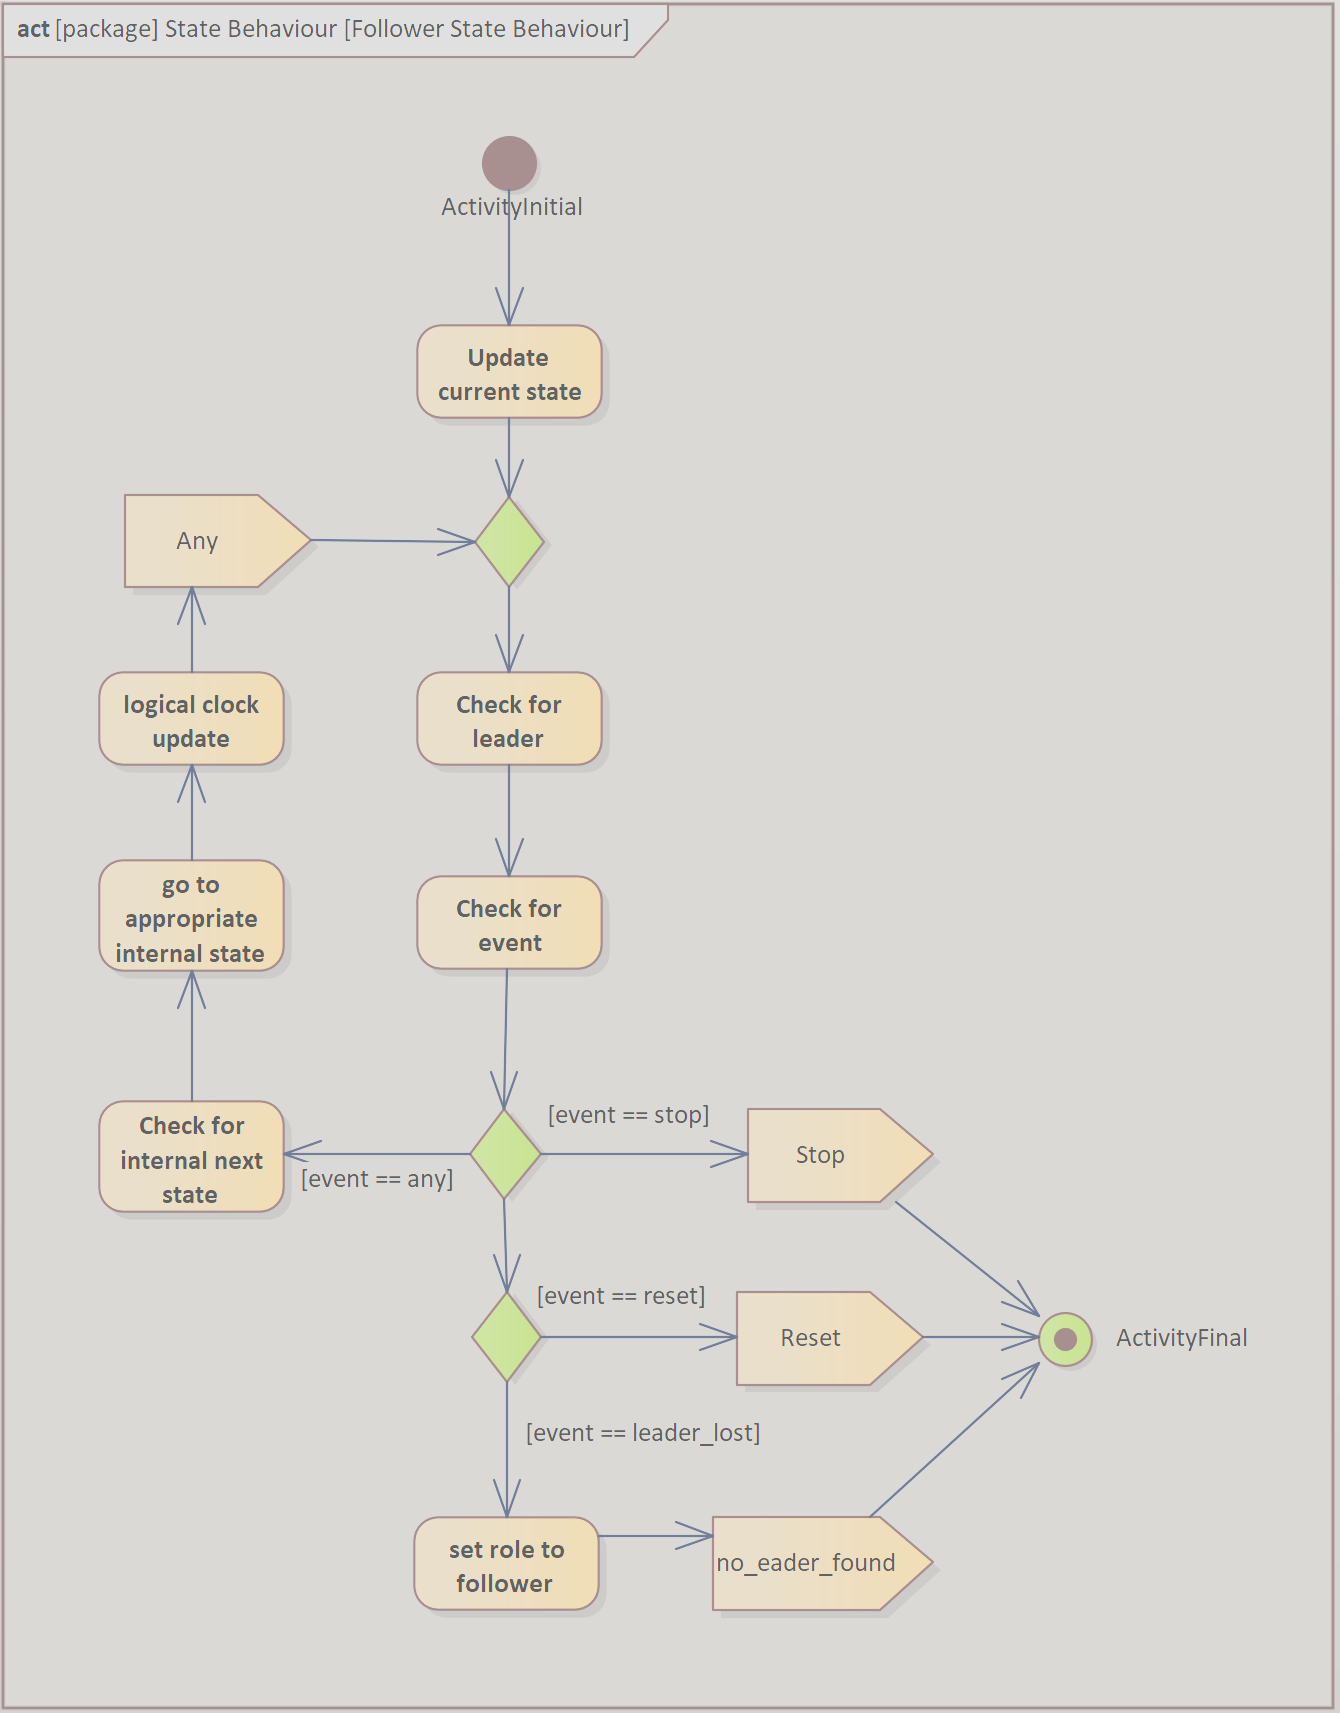
\includegraphics[width=0.4\textwidth]{images/follower_state_activity.png}
    \caption{ Follower state behaviour}
    \label{img:follower_state_activity}
\end{figure}

As follower, it will always wait for a new movement or an event from its leader. If none of them is received within a set time out, which is handled by a watchdog timer, a no\_leader\_found signal will be produced. Thus, the transition from follower state to the leader state will be triggered as in Figure \ref{img:controller_state_machine}. This shows the flexibility of trucks’ role.
In case the stop signal is received, the controller shall change its state to system stop state. For instance, when some of the vital component is not working that lead to Hazard (not visualized in this paper). For that reason, in the stop state, the controller tries to reset the truck.

%%% subsection Driver Interface
\subsection{Driver Interface}
\label{subsec:driver_interface}

%%% image driver interface
\begin{figure}[ht]
    \centering
    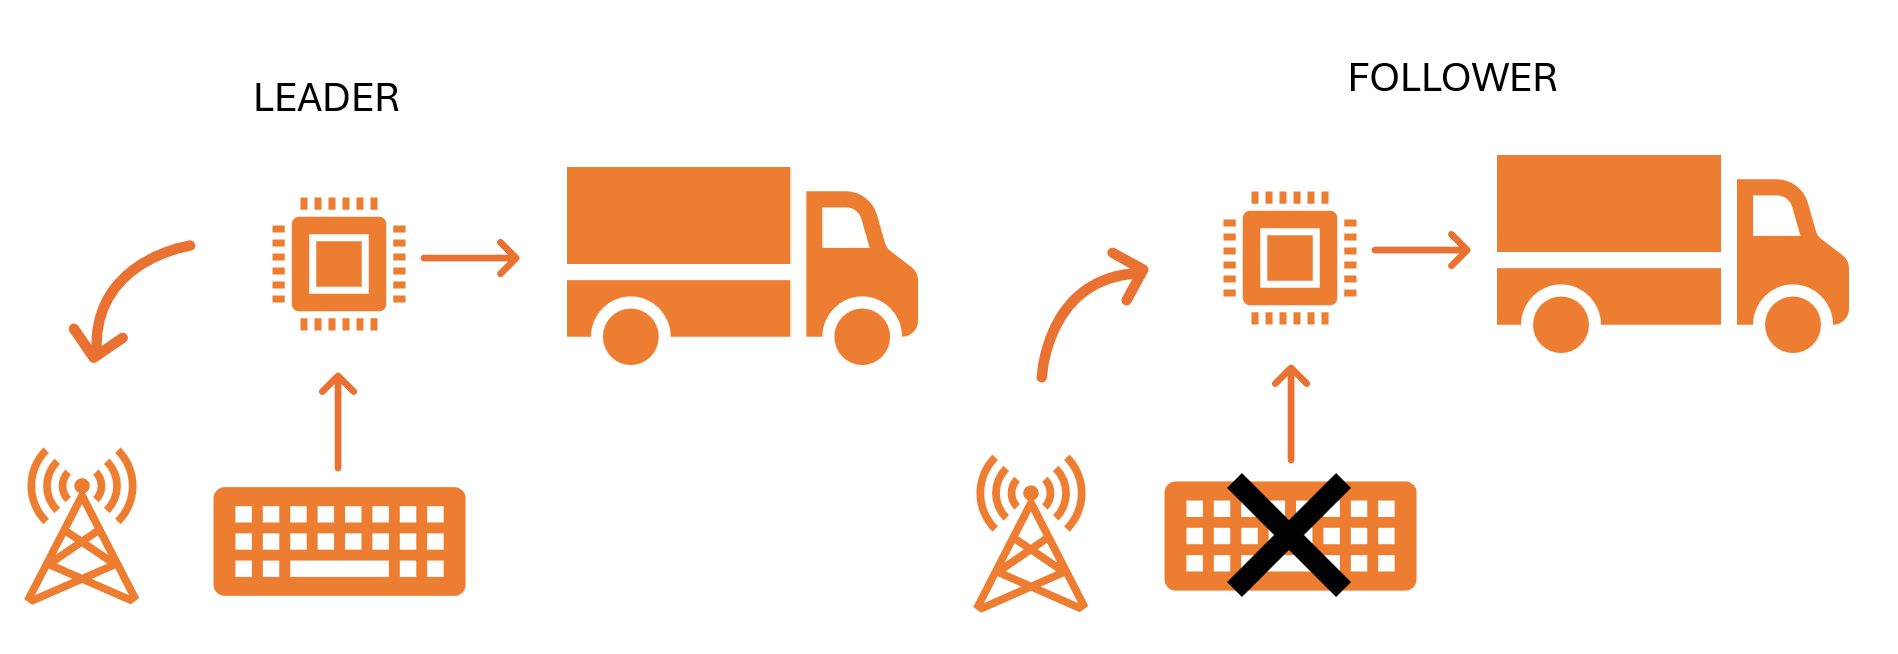
\includegraphics[width=0.5\textwidth]{images/DriverInterface.png}
    \caption{Basic input and output of the controller}
    \label{img:DriverInterface}
\end{figure}

The driver interface is the submodule that will allow us to interact with the system “Truck”. This interface is a basic user input using the keys “WASD” to increase or decrease the speed, in the case of “AD” key, it is just to select the direction of the truck, like a videogame. This to make the interaction as natural as possible. 
For the implementation of this user input the library “conio.h” was used, this because this library has a function to threat the input of the keyboard like an interruption. It will continue checking if an input was received from the keyboard, if this was the case then we will read this input and then send the information to the controller.
However, the input of the user will only be allowed in the case where the truck has the role of “LEADER” as in Figure \ref{img:DriverInterface}, in the other case, the input will simply be ignored. This behaviour is implemented as in Listing \ref{code:code_keyboard}.


%%% code key board input
\begin{lstlisting}[language = C++, caption=Driver interface only available for leader, label = code:code_keyboard]

if(self_truck->role == LEADER){
    inputChar = _getch();
}
else{
    inputChar;
}
\end{lstlisting}

%%% subsection Communication Module
\subsection{Communication Module}
\label{subsec:communication_module} 

The communication module is responsible for the communication between the truck and the server. This component will be explained more detailed in section \ref{sec:communication} where it will acts as a client.


%%% subsection Subsystem Collison Avoidance
\subsection{Collision Avoidance Subsystem}
\label{subsec:collition_avoidance}

Another subsystem of the truck that are handled by the controller is collision avoidance. This subsystem is to prevent any Hazard due to collision between the truck and the environment. One of the functionality of the system is to measure the distance of the obstacle around the truck and the truck itself. If the distance is below a threshold, the system shall raise a warning flag. For that reasons, we named this functionality distance validation. The behaviour of this functionality is modelled as in Figure \ref{img:distance_validation_activity}. There 4 distance there are measured in parallel as visualized in Figure \ref{img:distance_visual}. The red signal representing the distance is below threshold.

%%% image visual distance
\begin{figure}[ht]
    \centering
    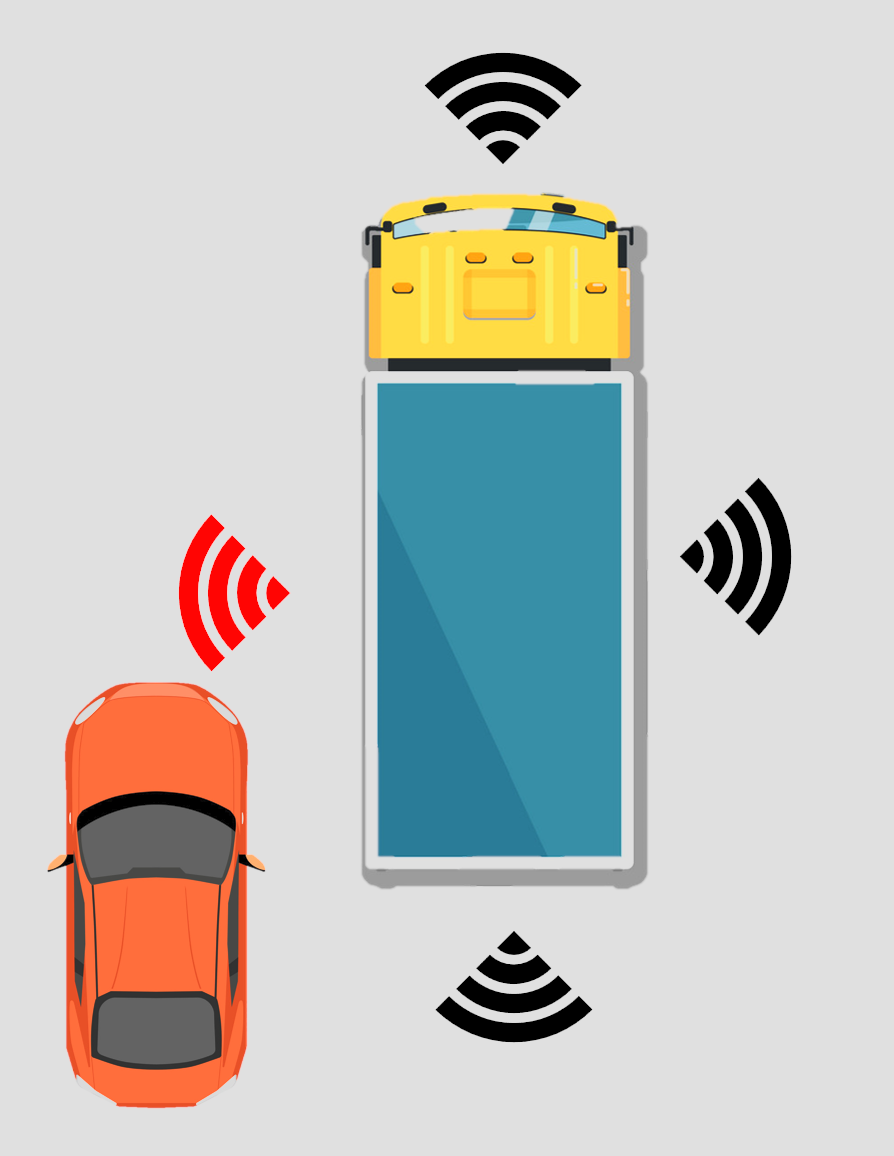
\includegraphics[width=0.2\textwidth]{images/distance_visual.png}
    \caption{Truck's sensor position}
    \label{img:distance_visual}
\end{figure}

%%% image distance validation
\begin{figure}[ht]
    \centering
    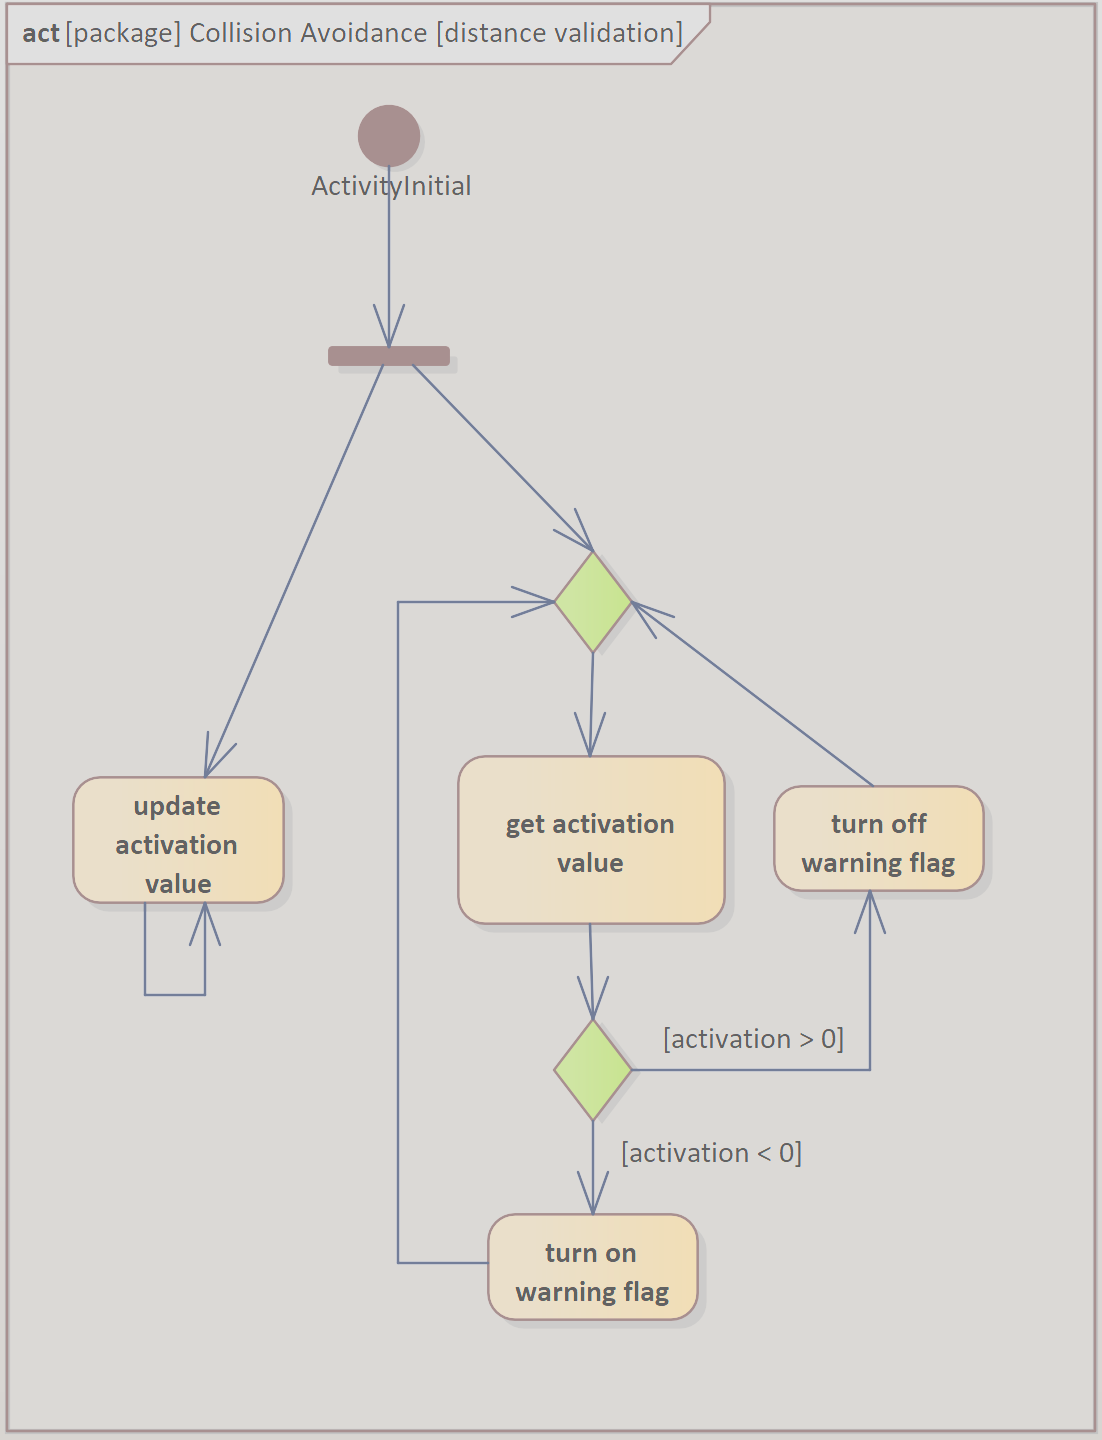
\includegraphics[width=0.3\textwidth]{images/distance_validation_activity.png}
    \caption{Distance validation activity}
    \label{img:distance_validation_activity}
\end{figure}

For safety reason, those distance shall validated in parallel that lead us to use GPU for parallel computation. In that case, we use Googlecolab GPU where the "update activation value" activity from Figure \ref{img:distance_validation_activity} is the kernel.
this computation consist of 3 array, sensor input, threshold and output. An example of the function use case is depicted in Figure

%%% image distance validation
\begin{figure}[ht]
    \centering
    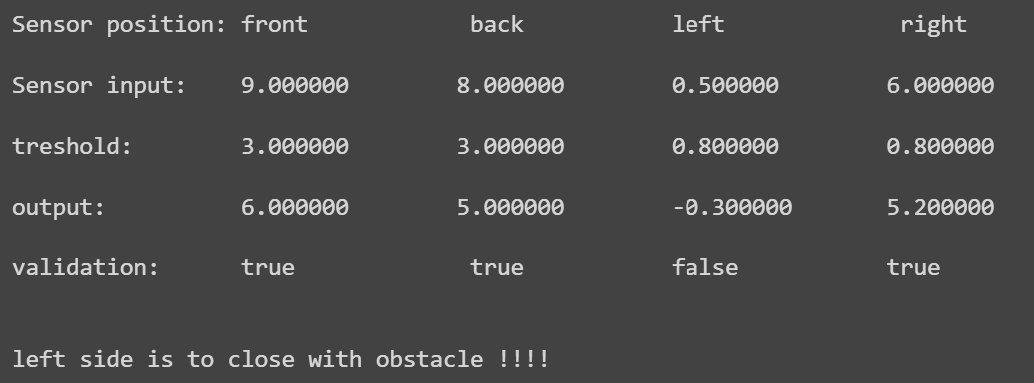
\includegraphics[width=0.5\textwidth]{images/distance_validation.png}
    \caption{Distance validation}
    \label{img:distance_validation}
\end{figure}












